\chapter{Aplicaciones en dimensión 2}%
\label{cha:aplicaciones_en_dimension_2_}
Veamos tres teoremas importantes que se pueden demostrar en dimensión $2$ con lo que ya hemos visto del grupo fundamental.

\section{Teorema fundamental del Álgebra}%
\label{sec:teorema_fundamental_del_algebra}
\begin{theo}[Fundamental del Álgebra]
Todo polinomio $P\left( z \right) \in \mathbb{C}\left[ z \right]$ tiene raíces complejas. 
\end{theo}
\begin{demo}
Sea $P\left( z \right) = z^d + a_1z^{d - 1} + \ldots + \overbrace{a_d}^{\neq 0}$ (mónico después de dividir por el cof. director)
\begin{enumerate}
    \item Tendremos:
    \begin{gather*}
        P_s\left( z \right) = z^d + sa_1z^{d - 1} + \ldots + sa_d = 0 \xRightarrow{0 \le s \le 1} \lvert z \rvert < 1 + \lvert a_1 \rvert + \ldots + \lvert a_d \rvert = r\\
        P_s \neq 0 \xRightarrow{z\neq 0} \text{entre } z^{d - 1}: -z = s\left( a_1 + \ldots + s \frac{a_d}{z^{d - 1}} \right) \Rightarrow \lvert z \rvert \le \begin{cases}
            1,\ \lvert z \rvert \le 1\\
            \lvert a_1 \rvert + \ldots + \lvert a_d \rvert,\ \lvert z \rvert \ge 1
        \end{cases} 
    .\end{gather*}

    \item $z\left( t \right) = r\left( \cos 2 \pi t, \sin 2 \pi t \right) \Rightarrow \lvert z \left( t \right)\rvert  = r \Rightarrow \exists H_s\left( t \right) = \frac{P_s\left( z\left( t \right) \right)}{\underbrace{\lvert P_s\left( z\left( t \right) \right) \rvert}_{\neq 0} }$ por 1.
    \begin{align*}
        \Rightarrow \left( \cos 2 \pi dt, \sin 2 \pi dt \right) &= \frac{z\left( t \right)^d}{\lvert z\left( t \right)^d \rvert} = H_0\left( t \right) \stackrel{\text{lazos: } z\left( 0 \right)= z\left( 1 \right)}{\simeq} H_1\left( t \right)\\
        &= \frac{P\left( z\left( t \right) \right)}{\lvert P\left( z \left( t \right) \right) \rvert} = \sigma\left( t \right) \Rightarrow d = \# \left( \ldots \right) = \# \sigma 
    .\end{align*}

    \item $P\left( z \right) \neq 0,\ \forall z \Rightarrow \exists G_s\left( t \right) = \frac{P\left( sz\left( t \right) \right)}{\lvert P\left( sz\left( t \right) \right) \rvert} : G_0 \equiv \frac{a_d}{\lvert a_d \rvert} \stackrel{\text{lazos}}{\simeq} G_1 = \sigma \Rightarrow 0 = \# \left( cte. \right) = \# \sigma$.
\end{enumerate}
\end{demo}

\section{Teorema del punto fijo de Brouwer}%
\label{sec:teorema_del_punto_fijo_de_brouwer}

\begin{theo}[de no retracto]
$\not \exists $ retracto $\rho: \mathbb{D}^2 = \{x^2 + y^2 \le 1\} \rightarrow \mathbb{S}^{1}$. 
\end{theo}
\begin{demo}
    Tenemos:
    \[
    \exists \rho \Rightarrow \rho_*: \overbrace{\underbrace{\pi\left( \mathbb{D}^2 \right) }_{\text{convexo}}}^{= \{0\}} \rightarrow \underbrace{\pi\left( \mathbb{S}^{1} \right)}_{\stackrel{\#}{=} \mathbb{Z}} \text{sobre (\ref{sec:retractos_y_deformaciones})
}   \]
\end{demo}

\begin{theo}[del punto fijo]
$\forall f: \mathbb{D}^2 \rightarrow \mathbb{D}^2$ continua, $\exists p$ punto fijo $x = f\left( x\right)$.
\end{theo}
\begin{demo}
Al absurdo?: $x \neq f\left( x \right), \forall x \Rightarrow \exists \rho: \mathbb{D}^2 \rightarrow \mathbb{S}^{1}$ retracto.

Construcción de $\rho$:
%TODO: Imagen
\begin{center}
    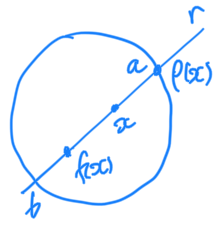
\includegraphics[scale=0.3]{images/construccion_rho_punto_fijo} 
\end{center}
La recta ($x \neq f\left( x \right)$), $r\left( x, f\left( x \right) \right) \cap \mathbb{S}^{1} = \{a, b\} \Rightarrow \rho\left( x \right) = a = x + \overbrace{\lambda \left( x \right)}^{> 0} \left( x - f\left( x \right) \right)$. 

\underline{Ejercicio}: Ecuación de $\lambda$ y continuidad.
\end{demo}

\section{Teorema de la esfera de Brouwer}%
\label{sec:teorema_de_la_esfera_de_brouwer}
\begin{theo}[de la esfera de Brouwer]
$\nexists \eta: \mathbb{S}^{2} \rightarrow \mathbb{R}^{3}$ campo tangente continuo sin ceros. (Tangente $\equiv \eta\left( x \right) \perp x,\ \forall x \in \mathbb{S}^{2}$)
\end{theo}
\begin{demo}
Con una ilustración:
%TODO: Imagen
\begin{center}
    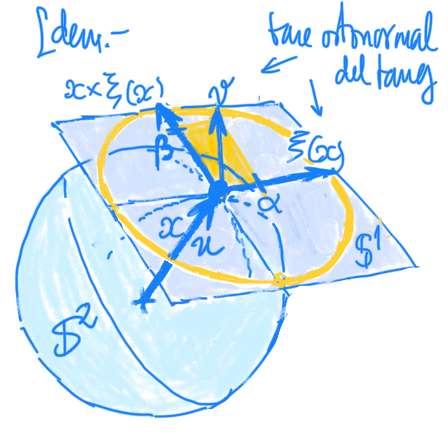
\includegraphics[scale=0.3]{images/dem_esfera_brouwer} 
\end{center}
Sea $\exists \eta$ sin ceros $\Rightarrow \exists \frac{\eta}{\lVert \eta \rVert}$ unitario $\Rightarrow$ podemos suponer $\lVert \eta \rVert = 1$:
\begin{enumerate}
    \item $h: \mathbb{S}^{1} \times \mathbb{S}^{2} \xrightarrow{\approx \text{ hom.}} SO\left( 3 \right) = $ \{matrices $3x3$ ortogonales, $\det > 0$\}
    \[
        \left( \alpha, \beta; x \right) \xmapsto{h} A = \left( u, v, u \times v \right) \begin{cases}
            u = x\\
            v = \alpha \eta\left( x \right) + \beta\left( x \times \eta\left( x \right) \right)
        \end{cases} 
    \]
    Con $\alpha^2 + \beta^2 = 1,\ \lVert x \rVert = 1$. Bien definida, continua y biyectiva $\xRightarrow{\text{compacto a } T_2}$ homeo.

    \item $h_*: \underbrace{\pi\left( \mathbb{S}^{1} \times \mathbb{S}^{2} \right)}_{= \mathbb{Z} \times \{1\}} \rightarrow \pi\left( SO\left( 3 \right) \right)$ isomorfismo $\Rightarrow \pi\left( SO\left( 3 \right) \right) = \mathbb{Z}$.

    %TODO: xd
    \item Abracadabra?: $SO\left( 3 \right) \stackrel{\text{homeo.}}{\approx} \mathbb{P}^{3} \Rightarrow \mathbb{Z} = \pi\left( SO\left( 3 \right) \right) = \pi \left( \mathbb{P}^{3} \right)$.
\end{enumerate}
\end{demo}


\chapter{Más aplicaciones por el mismo precio}%
\label{cha:mas_aplicaciones_por_el_mismo_precio}
Unos cuantos teoremas profundos más en $\dim = 2$.
\section{Borsuk-Ulam}%
\label{sec:borsuk_ulam}
\begin{theo}[de Borsuk]
Sea $f: \mathbb{S}^{1} \rightarrow \mathbb{S}^{1}$ impar $\left( f\left( -x \right) = -f\left( x \right) \right): \# f\left( \cos 2 \pi t, \sin 2 \pi t \right)$ impar ($\Rightarrow \# \neq 0$) 
\end{theo}
\begin{demo}
Tenemos que:
%TODO: Imagen
\begin{center}
    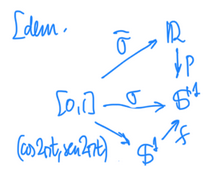
\includegraphics[scale=0.3]{images/th_borsuk} 
\end{center}
$\tilde{\sigma}$ elevación de $\sigma\left( t \right) = f\left( \cos 2 \pi t, \sin 2 \pi t \right)$. $\begin{cases}
    x = \left( \cos 2 \pi t, \sin 2 \pi t \right)\\
    0 \le t \le 1/2
\end{cases} (*)$.

$f\left( -x \right) = -f\left( x \right) \xRightarrow{(*)} \sigma\left( t + \frac{1}{2} \right) = -\sigma\left( t \right) \Rightarrow \tilde{\sigma} \left( t + \frac{1}{2} \right) = \tilde{\sigma} \left( t \right) + k_t + \frac{1}{2}$. Como $k_t \equiv cte.$ es continua:
\[
    \# \sigma = \tilde{\sigma} \left( 1 \right) - \tilde{\sigma} \left( 0 \right) = \left( \tilde{\sigma} \left( 1 \right) - \tilde{\sigma}{\left( \frac{1}{2} \right)} + \tilde{\sigma} \left( \frac{1}{2} \right) - \tilde{\sigma} \left( 0 \right) \right) = \left( \underbrace{k_{1/2}}_{k_0} + \frac{1}{2} \right) + \left( k_0 + \frac{1}{2} \right) = 2k_0 + 1
\]
\end{demo}

Análogamente, 
\begin{theo}[de Hirsch]
Sea $f: \mathbb{S}^{1} \rightarrow \mathbb{S}^{1}$ par $\left( f\left( -x \right) = f\left( x \right) \right): \# f\left( \cos 2 \pi t, \sin 2 \pi t \right)$ par. 
\end{theo}
\begin{coro}[Teorema de Borsuk-Ulam]
$f: \mathbb{S}^{1} \rightarrow \mathbb{S}^{1}$ impar $\Rightarrow$ esencial.
\end{coro}
\begin{demo}
$\exists H_s : f \simeq cte. \Rightarrow H_s\left( \cos 2 \pi t, \sin 2 \pi t \right) : \sigma \simeq x_0 \Rightarrow \# \sigma = 0$, con $\sigma$ rotación anterior y la homotopía de lazos.
\end{demo}
\begin{coro}[2]
$\nexists g: \mathbb{S}^{2} \rightarrow \mathbb{S}^{1}$ impar. 
\end{coro}
\begin{demo}
Tenemos:
%TODO: Imagen
\begin{center}
    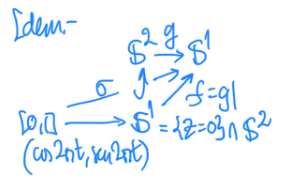
\includegraphics[scale=0.3]{images/cor_2_borsuk_ulam} 
\end{center}
\begin{itemize}
    \item $g$ impar $\Rightarrow f$ impar $\Rightarrow \# \sigma \neq 0$.

    \item $\mathbb{S}^{2}$ simple conexo $\exists H_s : \left( \cos 2 \pi t, \sin 2\pi t, 0 \right) \stackrel{\text{base } \left( 1, 0, 0 \right) \text{ fijo}}{\simeq} \left( 1, 0, 0 \right)$. Como $f = g\_{z = 0} \Rightarrow$
    \[
    g \circ H_s : f\underbrace{\left( \cos 2 \pi t, \sin 2 \pi t \right)}_{\sigma} \simeq f\left( 1, 0, 0 \right) cte. \Rightarrow \# \sigma = 0
    \]
\end{itemize}
\end{demo}
\begin{coro}[3]
$\forall h: \mathbb{S}^{2} \rightarrow \mathbb{R}^{2},\ \exists h\left( x \right) = h\left( -x \right) (\Rightarrow h$ no es 1-1).  
\end{coro}
\begin{demo}
$h\left( x \right) \neq h\left( -x \right),\ \forall x \Rightarrow \exists g \left( x \right) = \frac{h\left( x \right) - h\left( -x \right)}{\lVert h\left( x \right) - h\left( -x \right) \rVert}: \mathbb{S}^{2} \rightarrow \mathbb{S}^{1}$ impar.
\end{demo}

\section{Invarianza del dominio}%
\label{sec:invarianza_del_dominio}
\begin{theo}
Sea $f: U_{\text{ab.}} \rightarrow \mathbb{R}^{2}$ continua y 1-1 $\Rightarrow f\left( U \right)$ es abierto.
\end{theo}
\begin{demo}
$\forall a \in U,\ \exists V^{\text{ab.}} \subset \mathbb{R}^{2} : f\left( a \right) \in V \subset f\left( U \right)$. Por traslaciones: $a = f\left( a \right) = 0$. Con esto, $\exists \varepsilon > 0: $
\begin{align*}
    B\left( 0, \varepsilon \right) \subset B\left[ 0, \varepsilon \right] \subset U;\ &0 \not\in S = S\left[ 0, \varepsilon \right] \xRightarrow{\text{1-1}} 0 = f\left( 0 \right) \in f\left( S \right) \Rightarrow \exists V = C\left( 0 \right) \stackrel{\text{c.c}}{\subset} \mathbb{R}^{2} \setminus f\left( S \right) \\
    &S \text{ comp.} \Rightarrow f\left( S \right) \text{comp.} \Rightarrow \text{cerr. en } \mathbb{R}^{2} \\
    &\Rightarrow \mathbb{R}^{2} \text{loc. conx.} \Rightarrow V \stackrel[\text{conx.}]{\text{ab.}}{\subset} \mathbb{R}^{2} \Rightarrow \text{c. caminos}(*) 
.\end{align*}
Este $V$ es la solución: $V \subset f\left( B \right) \subset f\left( U \right)$.

Al absurdo: $\exists c \in V \setminus f\left( B \right) \xRightarrow{(*)} \exists \sigma: \left[ 0, 1 \right] \rightarrow V,\ \sigma\left( 0 \right) = c,\ \sigma\left( 1 \right) = 0$.

Denotamos, 
\[
g: \mathbb{S}^{1} \rightarrow\mathbb{R}^{2}: x \mapsto f\left( \varepsilon x \right);\ h: \mathbb{S}^{1} \rightarrow \mathbb{R}^{2}: x \mapsto g\left( x \right) - g\left( -x \right)
\]
y tenemos las homotopías: $\mathbb{S}^{1} \times \left[ 0, 1 \right] \rightarrow \mathbb{S}^{1}$.
\begin{itemize}
    \item $\frac{f\left( \varepsilon s x \right) - c}{\lVert \quad \rVert}: \frac{-c}{\lVert \ \rVert} \simeq \frac{g - c}{\lVert \ \rVert}$.
    \item $\frac{f\left( \varepsilon x \right) - \sigma\left( s \right)}{\lVert \quad \rVert}: \frac{g - c}{\lVert \ \rVert} \simeq \frac{g}{\lVert \ \rVert}$.
    \item $\frac{f\left( \varepsilon x \right) - f\left( -\varepsilon s x \right)}{\lVert \quad \rVert}: \frac{g}{\lVert \ \rVert} \simeq \frac{h}{\lVert \ \rVert}$
\end{itemize}
Con esto, $\frac{h}{\lVert \ \rVert} \simeq cte.$! por Borsuk-Ulam.

Que los denominadores no se anulan es una comprobación rutinaria.
\end{demo}

\section{Divarianza del borde y de la dimensión}%
\label{sec:divarianza_del_borde_y_de_la_dimension}
\begin{theo}
$S, T \subset \mathbb{R}^{2},\ h: S \stackrel{\text{homeo.}}{\approx} T \Rightarrow h\left( S \setminus \mathring{S} \right) = T \setminus \mathring{T}$.
\end{theo}
\begin{demo}
    $h: \mathring{S} \rightarrow \mathbb{R}^{2}$ inyectiva $\Rightarrow h\left( \mathring{S} \right) \stackrel[\ref{sec:invarianza_del_dominio}]{\text{ab.}}{\subset} \mathbb{R}^{2} \Rightarrow h\left( \mathring{S} \right) \subset \mathring{T}$. (el otro $\supset$ con $h^{-1}$)
\end{demo}

\begin{ej}
$S = T = \{x \ge 0\} \subset \mathbb{R}^{2} \Rightarrow h\left( x = 0 \right) = \left( x = 0 \right)$.    
\end{ej}

\begin{theo}
$U \stackrel{\text{ab.}}{\subset} \mathbb{R}^{n},\ V \stackrel{\text{ab.}}{\subset} \mathbb{R}^{2},\ h : U \stackrel{\text{homeo.}}{\approx} V \Rightarrow n = 2$.
\end{theo}
\begin{demo}
    $\exists H \subset \mathbb{R}^{n}$ [plano afín interior vacío en $\mathbb{R}^{n}$ salvo si $n = 2$](*) : $U \cap H \neq \emptyset \Rightarrow h| : \underbrace{U\cap H}_{\approx \text{ab.}} \xrightarrow{\text{1-1}} V \subset \mathbb{R}^{2} \xRightarrow{\ref{sec:invarianza_del_dominio}} h\left( U \cap H \right) \stackrel{\text{ab.}}{\subset} \mathbb{R}^{2} \xRightarrow{h \text{ homeo.}} U \cap H = h^{-1}h\left( U \cap H \right) \stackrel{\text{ab.}}{\subset } U \xRightarrow{(*)}
    n = 2$
\end{demo}

